\newpage
\chapter{ANALYSE DES SENTIMENTS ET DES EMOTIONS}


\vspace{15mm}


\textbf{Introduction}\par
L'analyse des sentiments et des émotions est une discipline de plus en plus essentielle dans le domaine de l'informatique et des sciences sociales. Ce chapitre se concentre sur une exploration approfondie de cette discipline, en mettant en évidence ses applications, son importance grandissante et les défis qu'elle présente.
\section{Analyse des sentiments et détection des émotions}
\subsection{Définition d'analyse des sentiments}
L’analyse des sentiments, également appelée extraction d'opinion, est un domaine de recherche qui analyse les opinions, les sentiments, les attitudes et les émotions des individus à l’égard des entités et de leurs attributs exprimés dans un texte écrit. Ces entités peuvent être des produits, des services, des organisations, des individus, des événements, ou des problèmes. Plusieurs termes connexes d’analyse des sentiments tels qu’extraction d'opinion, Analyse de subjectivité, Analyse des émotions, Analyse de l'affect, Extraction de critiques et Extraction d'évaluation \cite{liu2015mining}. \par
L'analyse des sentiments vise à identifier et prédire la tonalité d'un texte (positive ou négative), tout en explorant également les émotions sous-jacentes qui le sous-tendent, en utilisant des techniques et des mécanismes de traitement automatique et de langage naturel (NLP) afin de construire des outils qui soutiennent la prise de décision opérationnelle, managériale, et stratégique. \par
L’analyse des sentiments peut être effectuée à différents niveaux : l’analyse au niveau de document qui évalue le sentiment général d’un texte entier, l’analyse de la phrase qui identifie le sentiment de chaque phrase individuellement, et l’analyse au niveau des aspects qui identifie les sentiments relatifs à des aspects spécifiques d’un produit ou d’un service.
L’analyse des émotions, une sous-catégorie de l’analyse des sentiments, va au-delà de la simple polarité positive, négative ou neutre pour identifier des émotions plus complexes telles que la joie, la tristesse, la colère, la peur et l’amour.     

\subsection{Importance de l'analyse des sentiments}
L’analyse des sentiments et des émotions est essentielle dans tous les secteurs qui fonctionnent grâce à l’interaction humaine en tant qu’outil de gestion des risques, elle facilite la compréhension des émotions et la prise des décisions. Voici quelques utilisations de l’analyse des sentiments \cite{tweetEraser2024}: \par
\textbf{La satisfaction des clients:} les marques et les entreprises reçoivent souvent de nombreux avis de clients via leurs comptes sur les réseaux sociaux, ces entreprises peuvent se brancher sur l’écoute sociale et analyser ce vaste ensemble de données. Ce processus permet de comprendre l’opinion des clients sur les activités, les produits, et les services qu’ils présentent, ainsi grâce à l’évaluation des sentiments, on peut savoir si les produits et services d’une marque satisfont le public. Les entreprises peuvent utiliser également l’analyse des opinions pour améliorer leurs services d’assistance clientèle, ils peuvent découvrir quelles sont les demandes les plus urgentes et y répondre en priorité, de cette manière, ils peuvent maintenir la satisfaction de leurs clients. \par
\textbf{L’étude de marché:} auparavant, on préparait des questionnaires et des enquêtes pour obtenir le point de vue des clients afin de déterminer les préférences de public et de consommateurs. Ce processus n’était pas facile, parce qu’il prend beaucoup de temps et les clients ne répondent pas toujours sérieusement aux questions. Maintenant, grâce aux réseaux sociaux, les entreprises pourraient facilement s’engager dans l’écoute sociale à l’aide d’un modèle d’analyse des sentiments et de détection des opinions qui est utile pour dégager les tendances de marché et les besoins des clients. \par
\textbf{Conservation de réputation:} l’analyse des sentiments aide les sociétés à gérer les risques et à concevoir leur réputation en surveillant les sentiments exprimés sur les réseaux sociaux, une seule mauvaise critique peut nuire à la réputation de l’entreprise, rendant toutes les stratégies de marketing et de publicités inutiles. Mais grâce à l’analyse des sentiments en temps réel, les marques peuvent recevoir les opinions négatives et prendre des mesures rapides pour limiter ces critiques avant qu’elles ne deviennent incontrôlables.\par  
\textbf{L’étude politique :} l’analyse des sentiments joue un rôle crucial dans le monde politique, les politiciens et les analystes peuvent examiner les opinions et les émotions exprimées sur des plateformes comme Twitter (alias X), pour obtenir des insights précieux sur l’état de l’opinion publique. Aussi, le pouvoir législatif et judiciaire peut suivre la réaction de la population aux nouvelles lois.\par
En résumé, l'analyse des sentiments et des émotions est un outil puissant pour les entreprises et les institutions, leur permettant de mieux comprendre et répondre aux besoins et aux opinions des individus.


\subsection{Applications de l’analyse des sentiments}
Les applications d’analyse des sentiments et des émotions sont nombreuses, touchent plusieurs domaines \cite{duwairi2014sentiment}:
\begin{itemize}
    \item \textbf{Marketing:} les médias sociaux sont devenus une plateforme unique d’interaction avec les clients, l’utilisation de l’analyse des sentiments peut facilement amener le marketing à un autre niveau, il est utilisé à comprendre les perceptions des clients à l’égard d’une marque, d’un produit ou d’un service et prendre des décisions éclairées et améliorer l'expérience globale des consommateurs.
    \item \textbf{Finance:} avec l’analyse des sentiments, les investisseurs surveillent les conversations sur les réseaux sociaux pour détecter les tendances émergentes et évaluer le sentiment de marché en temps réel, par exemple, ils peuvent analyser les tweets des traders et des analystes financières pour évaluer l’optimisme et le pessimisme à l’égard d’une action spécifique afin de prendre des meilleures décisions financières.
    \item \textbf{Santé:} l’analyse des sentiments peut également être utilisée dans le monde de la santé, les blogs médicaux sont partout sur Internet, ces blogs que des sujets médicaux et de santé, telle que les maladies, les traitements médicaux et les médicaments. En raison des expériences liées à la santé et des antécédents médicaux que ces pages web fournissent aux praticiens et aux patients, des outils d'analyse des sentiments ont dû être développés pour une utilisation dans les domaines médicaux.
    \item \textbf{La politique: }les retours d'information des médias sociaux ont été utilisés pour informer les dirigeants politiques des menaces potentielles, des problèmes ou des questions avec leurs organisations. De plus, un rôle essentiel pour l'analyse des sentiments est apparu plus tôt dans la prédiction des élections, et dans l'obtention des réponses des citoyens sur des questions importantes telles que l'augmentation des prix et la modification de la constitution.
\end{itemize}









%%%%%%%%%%%%%%%%%%%%ù NLP  %%%%%%%%%%%%%%%%%%%%%%ù 
\section{Traitement du langague automatique (NLP)}
Le traitement automatique de langage naturel NLP est une branche de l’intelligence artificielle qui s’attache à donner la capacité aux machines de comprendre, générer ou traduire les langages humains tel qu’il est écrit et/ ou parlé \cite{journaldunet2022nlp}. \par
NLP est un domaine multidisciplinaire combinant la linguistique informatique (modélisation du langage humain basée sur des règles) avec des modèles statistiques et des modèles de machine learning, il est utilisé pour la construction des applications et des systèmes permettant l’interaction entre les machines et les langages naturels crée par les humains. 


%%%%%%%%%%%%%%%%%%%%%%%%%%%%%ù HISTORIQUE %%%%%%%%%%%%ù
\subsection{Histoire et évolution de NLP}
Le domaine du traitement automatique du langage naturel (TALN) a commencé à émerger dans les années 1950 aux États-Unis. Le test de Turing fut la première application liée au traitement automatique de la conversation, tel que décrit par Alan Turing en 1950 dans sa publication "Computing Machinery and Intelligence" \cite{wikipediaTuringTest}.\par
Le psychologue Joseph Weizenbaum a développé ELIZA, souvent cité comme le premier programme de traitement automatique du langage capable de mener des conversations simples \cite{frenchwebEliza}. Dans les années 1970-1980, la recherche sur la compréhension du langage naturel a continué avec des systèmes comme SHRDLU, développé par Terry Winograd, permettant aux utilisateurs d'interagir avec un ordinateur dans un monde de blocs \cite{mediumShrdlu}. \par
À partir de l'an 2000, l'essor du Big Data et des algorithmes plus avancés tels que les réseaux neuronaux a permis des avancées significatives dans le TALN. De 2010 à aujourd'hui, les modèles de traitement automatique du langage naturel ont connu une révolution avec l'introduction de réseaux neuronaux profonds et d'autres architectures.

%%%%%%%%%%%%%%%%%%%%%%%%%%ù NLP PROCESS %%%%%%%%%%%%
\subsection{Processus de traitement}
Le processus de traitement automatique de langage naturel (Voir la figure[\ref{fig:figureProcess}]) est une discipline qui peut être divisé en deux parties principale, la première partie est la compréhension de langage naturel par la définition de l’entrée donnée en langage naturel en une représentation utile et analyse de différents aspects de la langue, la deuxième partie est la génération de langage naturel, qui concerne la planification de texte (récupération de contenu pertinent de la base de connaissances) et planification de la phrase (la formation des phrases significatives).
\begin{figure}[h]
    \centering
    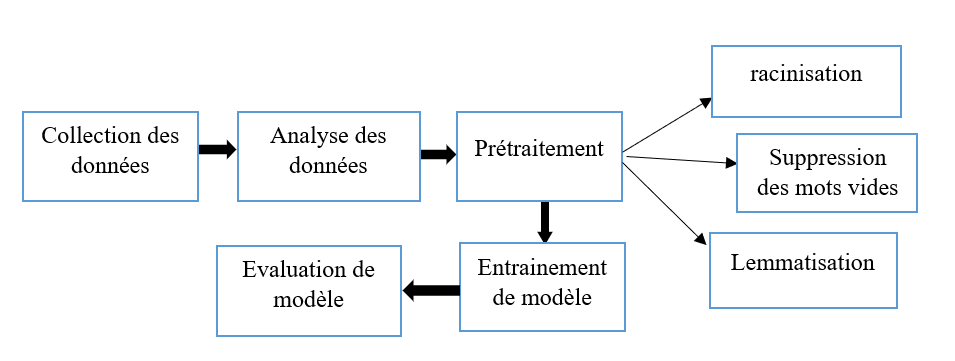
\includegraphics[width=0.9\textwidth]{project_report/figures/Capture d’écran (689).png} 
    \caption{\textit{Processus du traitement de langage naturel \cite{technoaretepublication}.}}
        \label{fig:figureProcess}
 
\end{figure}

%%%%%%%%%%%%%%%%%ù NLP APP %%%%%%%%%%%%%%%%%
\subsection{Domaine d'application}
Le traitement de langage naturel est le moteur de l’intelligence artificielle, avec des applications pratiques variées dans le monde actuel comme \cite{ibmNLP}:
\begin{itemize}
    \item \textbf{Traduction automatique:} Google Translate est un exemple couramment utilisé le traitement automatique de langage naturel (TALN). Une traduction efficace va au-delà du simple remplacement de mots d'une langue à une autre ; elle doit transmettre avec précision le sens et le ton du texte original dans la langue cible. La qualité des outils de traduction automatique s'améliore continuellement. Un bon test pour ces outils est de traduire un texte dans une autre langue, puis de le traduire à nouveau dans la langue d'origine. Par exemple, il y a quelques années, la phrase "The spirit is willing but the flesh is weak" traduite en russe puis en anglais donnait "The vodka is good but the meat is rotten." Aujourd'hui, la traduction inverse donne "The spirit desires, but the flesh is weak," montrant une amélioration notable, bien que ce ne soit pas encore parfait.
    \item \textbf{Agents virtuels et chatbots:} Les assistants virtuels comme Siri d'Apple et Alexa d'Amazon utilisent la reconnaissance vocale pour détecter des schémas dans les commandes vocales et la génération de langage naturel pour fournir des réponses appropriées. De même, les chatbots répondent aux textes saisis par les utilisateurs. Les meilleurs de ces systèmes apprennent à reconnaître des indices contextuels dans les demandes des utilisateurs, ce qui leur permet d'offrir des réponses de plus en plus pertinentes. Une prochaine avancée dans ce domaine est la réponse aux questions, où les systèmes pourront fournir des réponses pertinentes et utiles de manière proactive.
    \item \textbf{Résumé de texte:} Le résumé de texte emploie des techniques de TALN pour condenser de grands volumes de texte numérique en résumés ou synopsis. Cela est utile pour les index, les bases de données de recherche, ou pour les lecteurs pressés. Les meilleurs outils de résumé de texte utilisent le raisonnement sémantique et la génération de langage naturel pour ajouter du contexte et des conclusions pertinentes aux résumés.
\end{itemize}

%%%%%%%%%%%%%%%%%%%%ù APPROCHES %%%%%%%%%%%%%%
\section{Approches d'analyse des sentiments et des émotions}
L'analyse des sentiments repose sur plusieurs approches pour extraire et comprendre les émotions et les opinions dans un texte. Ces approches incluent (Voir la figure [\ref{fig:figure7}]): approche par lexique, approche hybride et approche basée sur le machine learning. Ces approches seront explorées en détail dans les sous-sections suivantes, mettant en lumière leurs avantages, leurs limitations et leurs applications spécifiques.

\begin{figure}[h]
    \centering
    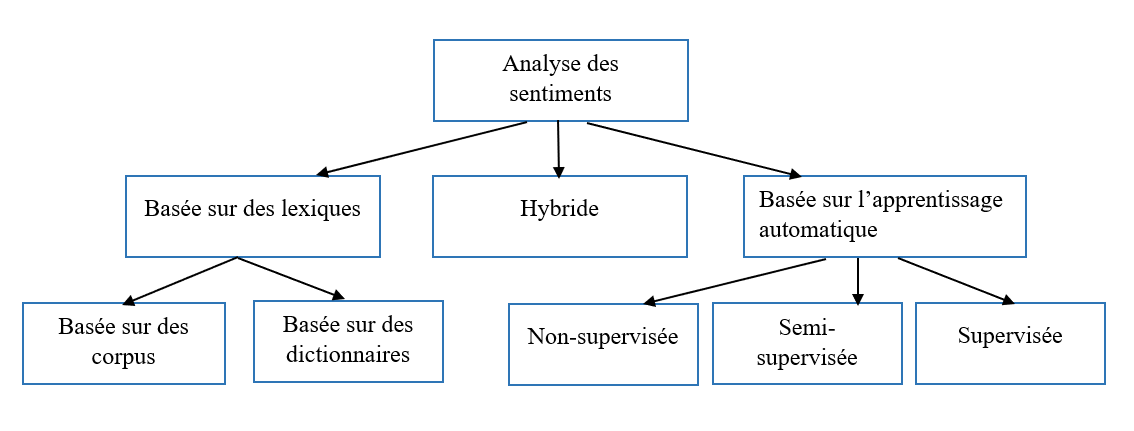
\includegraphics[width=1\textwidth]{project_report/figures/Capture d’écran (690).png} 
    \caption{\textit{Approches d'analyse des sentiments et des émotions }.}
        \label{fig:figure7}
 
\end{figure}

\subsection{Approche basée sur le machine learning}
L’approche de l’apprentissage automatique pour l’analyse des sentiments implique plusieurs étapes. Les données collectées à partir des diverses sources sont préretraitées en supprimant les mots vides pour l’élimination de bruit et la standardisation de format, les caractéristiques pertinentes sont alors extraites sous forme des vecteurs des mots à l’aide des techniques de représentation textuelle telles que le sac de mot ou TF-ID. Un algorithme de classification (régression logistique, les machines à vecteurs de support SVM, les réseaux de neurones...) choisi et entraîné sur l’ensemble des données, il apprend à associer certaines caractéristiques à des sentiments positifs, négatifs ou neutre et à des émotions de joie, de surprise, de peur..., afin d’être capable de classifier des nouveaux textes.  

%%%%%%%%%%%%%ùù LEXICAL APPROCHES %%%%%%%%%%
\subsection{Approche lexicale}
Une Méthode basée sur le lexique, elle repose sur l’utilisation des dictionnaires (Voir la figure [\ref{fig:figure7}], couramment utilisée en analyse des sentiments et dans l’autre application de NLP. \par
Un exemple populaire de modèle d'analyse de sentiment basé sur le lexique en Python est TextBlob. C’est une bibliothèque Python basée sur le Natural Language Toolkit (NLTK) qui calcule le score de sentiment pour les textes. Une technique de moyennage est appliquée à chaque mot pour obtenir les scores de polarité des sentiments pour l'ensemble du texte. \par
Les mots enregistrés dans le lexique de TextBlob ont leur score de polarité correspondant, score de subjectivité et score d'intensité. De plus, il peut y avoir différents enregistrements pour le même mot, donc le score de sentiment du mot est la valeur moyenne de la polarité de tous les enregistrements le contenant.

%%%%%%%%%%%%%ù HYBRIDE APPROCHE %%%%%%%%%%%
\subsection{Approche hybride}
L’approche hybride combine des méthodes basées sur le lexique (Voir la figure [\ref{fig:figure7}]) avec des techniques d’apprentissage automatique. Cette approche en analyse des sentiments permet d’obtenir des résultats plus précis et robustes en combinant les forces des méthodes basées sur le lexique et des techniques d’apprentissage automatique, elle offre une adaptabilité accrue et efficace pour le traitement des textes variés et complexes dans différents domaines.


%%%%%%%%%%%%%%%%%%ùù SENTIMENT ANALYSIS AND TWITTER %%%%
\section{L'analyse des sentiments et Twitter}





%%%%%%%%%%%%%%%%%%%%%% TWITTER %%%%%%%%%%%
\subsection{Twitter et ses attouts}
\textit{Twitter} fondé le 21 Mars 2006 et renommé \textit{X }en juillet 2023 est un réseau social de microbloguage, il permet aux utilisateurs de publier des messages courts qui ne dépassent pas 280 caractères (tweets), cette plateforme a connu une croissance régulière ces dernière années, est devenue un instrument incontournable de communication pour tous les acteurs sociaux (les hommes politiques, les sportifs, les dirigeants d’entreprise…) qui l’utilisent pour partager leurs actualités, leurs décisions, et leurs actions à venir. Twitter ou bien X constitue également une plateforme d’échange qui permet à tous d’exprimer son opinion en réaction à une annonce ou un événement, ce qui en fait un outil indispensable pour les personnes qui cherchent à comprendre les schémas de pensées des humaines.

%%%%%%%%%%%%%%%%%%%%% LATEST RESEARCH %%%%%%%%%%%%
\section{Travaux Connexes}
L'étude de l'analyse des sentiments est un domaine de recherche qui a suscité beaucoup d'intérêt. Les travaux antérieurs dans ce domaine se concentrent sur le développement des déverses méthodes et algorithmes pour classer les avis en catégorie telle que positive, négative, ou neutre. \par
La première approche était présentée par Hu et lui (2004), cette approche est basée sur l’analyse de la polarité pour classer les textes en fonctions de leur sentiment, l’objectif principal de hu et lui dans leur travail est de fournir aux consommateurs et aux entreprises des résumés utiles et des informations agrégées à partir des avis des clients afin de faciliter la prise de décision. Cette contribution à démontré aussi que l’incorporation des caractéristiques linguistiques spécifiques à Twitter (émoticônes, hashtags) pourrait améliorer les performances des modèles \cite{hu2004mining}. \par
Avec l’évolution des techniques d’apprentissage automatique, des algorithmes plus sophistiqués ont été appliqués. Par exemple Pak et Paroubek (2010) proposent différentes approches pour l’analyse des sentiments sur Twitter, alias X, des techniques de classification supervisée tels que Naïve Bayes et SVM et des méthodes basées sur l’apprentissage non supervisés (clustering) utilisés pour l’entraînement des modèles d’analyse de sentiments des tweets, Park et Paroubek évaluent également les performances de ces techniques, en mettant en lumière les caractéristiques uniques de Twitter et en proposant des approches pour relever les défis associés à l’analyse des sentiments sur cette plateforme \cite{pak2010twitter}. \par
De même, ils existent des marques, des entreprises et des organisations qu’ont un intérêt commercial auquel pourrait service un système autonome d’analyse des sentiments. L’étude menée par Rui, Liu et Whinston (2013) explore l’impact des tweets sur les ventes des billets de cinéma pour les films nouvellement sortis. Les résultats de cette étude ont montré que les tweets positifs étaient fortement corrélés avec une augmentation des ventes des billets de cinéma, tandis que les tweets négatifs avaient un effet dissuasif sur les ventes, ce qui suggère que la surveillance des sentiments sur Twitter peut fournir des indications précieuses sur les performances commerciales d’une entreprise \cite{rui2013whose}.  \par            
L’évolution de l’analyse des sentiments présente aussi ces dernières années un potentiel intéressant dans le domaine de la santé. Dans ce contexte, l’exploitation des données provenant de Twitter peut fournir des informations précieuses sur les expériences et les émotions des patients. Un exemple notable est l’étude menée par Crannell et Al (2016) sur le comportement d’utilisation de Twitter chez les survivants de cancer. Dans cette étude Crannell et Al ont collecté et analysé des tweets contenant des hashtags populaires liés au cancer. L’objectif principal était de comprendre les émotions dominantes exprimées chez les patients de cancer. Cette contribution a des implications importantes pour la communauté des patients et les organisations de la santé, car il met en évidence l’importance de soutien émotionnel sur le web. De plus, elle montre comment l’analyse des sentiments sur Twitter peut fournir des insights précieux pour comprendre les expériences des patients et améliorer les interventions de soutien \cite{crannell2016cancer}.

%%%%%%%%%%%%%%%%%% LIMITS  %%%%%%%%%%%%%%
\section{Défis et limitations d'analyse des sentiments et des émotions}
Malgré le progrès des technologies de langage de traitement automatique NLP, la compréhension de langage humaine est encore compliquée pour les machines:

%%%%%%%%%%%%%%%%%  SARCASME & IRONIE %%%%%%%%%%%%
\subsection{Sarcasme et Ironie}
Les expressions sarcastiques ou ironiques peuvent être difficiles à détecter par les modelés d’analyse des sentiments et des émotions, car ces expressions impliquent toujours un sens figuré ou inversé. Par exemple, « Bravo, tu as vraiment fait un travail formidable en oubliant de faire tes devoirs. »
Le modèle n’analyse pas la phrase avec une compréhension complète de scénario, il qualifiera l’expérience de positive sur la base de mots ‘Bravo’.  


%%%%%%%%%%%%%%%%%%%%%%ùù SUBJECTIVITE %%%%%%%%%%%%%%
\subsection{Subjectivité et Ambiguïté}
 L’analyse des sentiments peut rencontrer des difficultés avec des phrases subjectives et ambiguës. Les opinions et les sentiments exprimés sont parfois intrinsèquement subjectifs, ce qu’est perçu comme positif par une personne, peut être négatif par une autre. Par exemple, « le service était rapide mais impersonnel » peut refléter un sentiment mitigé ou équilibré en fonction des attentes et des critères de l’évaluateur. De même, le langage humain est souvent ambigu avec des phrases et des mots qui peuvent avoir plusieurs significations. Par exemple, « la présentation était intense » pourrait être interprétée positivement (comme une présentation intéressante) ou négativement (comme une présentation négative).     

 %%%%%%%%%%%%%%%%%%%%%%%%%%% MULTIPOLARITE %%%%%%%%%%
 \subsection{Multipolarité}
 La multipolarité consiste à identifier et à interpréter plusieurs sentiments contradictoires exprimés simultanément dans le même texte, elle présente un défi majeur pour les modèles d’analyse des sentiments. Un commentaire peut contenir des sentiments positifs et négatifs au même temps, par exemple « j’adore la qualité de caméra, mais la batterie est horrible », cette phrase contient deux opinions sur la qualité de produit (positive) et sur la batterie (négative), cette multipolarité rend l’analyse des sentiments plus complexe, car c’est difficile de distinguer à quelle classe le modèle doit ajouter cette phrase (positive, négative, ou neutre).
Ce qui nécessite des algorithmes avancés capable de traiter le contexte et de comprendre les nuances linguistiques.


%%%%%%%%%%%%%%%%%%%%%%%%%%%%% EVOLUTION DE LANGAGE %%%%
Le langage humain est une entité qui évolue rapidement et constamment, surtout dans le monde de web et des réseaux sociaux, des nouveaux mots, des expressions et des formes de communication émergent régulièrement, par exemple \textit{Twitter} ou bien \textit{X} voient naître des néologismes, des hashtags qui peuvent rapidement devenir des vecteurs importants d’opinions et d’émotions. Dans ce cadre, les modèles d’analyse des sentiments et de détection des émotions doivent être continuellement mis à jour pour intégrer ces nouveautés, non seulement par la collecte des nouvelles données, mais aussi par l’adaptation des nouveaux algorithmes de traitement. Jacob Eisenstein dans son article «\textit{ what to do about bad language on the internet} » écrit en 2023, souligne ce défi et propose des méthodes pour adapter les modèles aux changements linguistiques en temps réel \cite{eisenstein2013bad}.

\textbf{Conclusion}\par
En résumé, ce chapitre offre une plongée profonde dans le monde de l'analyse des sentiments et des émotions, mettant en lumière son rôle central dans notre société numérique moderne et explorant les opportunités et les défis qui l'accompagnent.






